% Created 2014-11-09 Sun 16:59
\documentclass[table]{beamer}
\usepackage[T1]{fontenc}
\usepackage{fixltx2e}
\usepackage{graphicx}
\usepackage{longtable}
\usepackage{float}
\usepackage{wrapfig}
\usepackage{soul}
\usepackage{textcomp}
\usepackage{marvosym}
\usepackage{wasysym}
\usepackage{latexsym}
\usepackage{amssymb}
\usepackage{hyperref}
\tolerance=1000
\usepackage{etex}
\usepackage{amsmath}
\usepackage{pstricks}
\usepackage{pgfplots}
\pgfplotsset{compat=1.8}
\usepackage{tikz}
\usepackage[europeanresistors,americaninductors]{circuitikz}
\usepackage{colortbl}
\usepackage{yfonts}
\usetikzlibrary{shapes,arrows}
\usetikzlibrary{positioning}
\usetikzlibrary{arrows,shapes}
\usetikzlibrary{intersections}
\usetikzlibrary{calc,patterns,decorations.pathmorphing,decorations.markings}
\usepackage[BoldFont,SlantFont,CJKchecksingle]{xeCJK}
\setCJKmainfont[BoldFont=Evermore Hei]{Evermore Kai}
\setCJKmonofont{Evermore Kai}
\usepackage{pst-node}
\usepackage{pst-plot}
\psset{unit=5mm}
\usepackage{beamerarticle}
\mode<beamer>{\usetheme{Frankfurt}}
\mode<beamer>{\usecolortheme{dove}}
\mode<article>{\hypersetup{colorlinks=true,pdfborder={0 0 0}}}
\mode<beamer>{\AtBeginSection[]{\begin{frame}<beamer>\frametitle{Topic}\tableofcontents[currentsection]\end{frame}}}
\setbeamercovered{transparent}
\subtitle{频率分析介绍}
\mode<article>{\renewcommand{\labelitemii}{$\cdot$}}
\providecommand{\alert}[1]{\textbf{#1}}

\title{线性系统的频域分析法}
\author{邢超}
\date{}
\hypersetup{
  pdfkeywords={},
  pdfsubject={},
  pdfcreator={Emacs Org-mode version 7.9.3f}}

\begin{document}

\maketitle

\begin{frame}
\frametitle{Outline}
\setcounter{tocdepth}{3}
\tableofcontents
\end{frame}










\section{频率法介绍}
\label{sec-1}
\subsection{频率法基本概念}
\label{sec-1-1}
\begin{frame}
\frametitle{频域法特点:}
\label{sec-1-1-1}

\begin{enumerate}
\item <2->工程使用广泛,有自己一套指标体系
\item <3->时域与频域指标可由经验公式相互转化
\item <4->根据Nyquist判据可由系统的开环频率特性判断闭环系统的稳定性,频率特性可由实验测定
\item <5->频率特性还可适用于典型非线性环节系统
\item <6->可以方便地设计出各种滤波器
\end{enumerate}
\end{frame}
\begin{frame}
\frametitle{频率特性基本概念}
\label{sec-1-1-2}
\begin{itemize}

\item RC网絡:\\
\label{sec-1-1-2-1}%
\begin{circuitikz}[american voltages,scale=0.7]
%       o---R --+-------o
%               |
%      U_r   C ===      U_c
%               |
%       o-------+-------o
\draw
  % rotor circuit
  (0,0) to  [short, o-o] (5,0)
  to [open, v^>=$U_c$ ,-o](5,3)
  to [short] (3,3)
  to [C, l_=$C$] (3,0)

  (0,0) to [open, v>=$U_r$ ,-o] (0,3)
  to [R,l=$R$] (3,3);
\end{circuitikz}

\begin{eqnarray*}
U_r &=& U_c + RC\dot{U}_c \\
U_r(s) &=& U_c(s) + RsU_c(s) 
\end{eqnarray*}


\item 传递函数:
\label{sec-1-1-2-2}%
\begin{eqnarray*}
%U_r &=& U_c + RC\dot{U}_c \\
%U_r(s) &=& U_c(s) + RsU_c(s) \\
G(s) &=& \frac{U_c(s)}{U_r(s)} \\
   &=&\frac{1}{1+RCs} \\
  &=& \frac{1}{1+Ts} 
\end{eqnarray*}
其中, $T=RC$ ,

\end{itemize} % ends low level
\end{frame}
\begin{frame}
\frametitle{频率特性基本概念(续)}
\label{sec-1-1-3}

\begin{itemize}
\item <2->当 $U_r=A\sin\omega t$ 时,
         \begin{eqnarray*}
         U_c(s) & =& G(s)U_r(s)\\
         U_c(t) &=& \frac{A\omega t}{1+\omega^2 T^2}e^{-\frac{t}{T}}+\frac{A}{\sqrt{1+\omega^2 T^2}}\sin(\omega t-\beta)
         \end{eqnarray*}
\item <3->稳态分量为 
       \[\frac{A}{\sqrt{1+\omega^2 T^2}}\sin(\omega t-\beta)\]
       	其中, $\tan\beta=\omega T$ .
\item <4->结论:
\begin{itemize}
\item <4->对线性系统而言,输入为正弦信号,输出也为相同频率的正弦信号,但幅值与相位发生变化.
\item <5->幅值变化:输出是输入的  $\frac{1}{\sqrt{1+\omega^2 T^2}}$  倍
\item <6->相角变化:输出比输入滞后  $\arctan \omega T$  .
\end{itemize}
\end{itemize}
\end{frame}
\begin{frame}
\frametitle{频率特性定义}
\label{sec-1-1-4}

\begin{itemize}
\item <2->幅频特性:系统稳态正弦输出量与输入量的幅值比  $A(\omega)$
\item <3->相频特性:系统稳态正弦输出量与输入量的相角差  $\phi(\omega)$
\item <4->令  $s=j\omega$  ,则
       \begin{eqnarray*}
       A(j\omega)&=&|G(j\omega)|  \\
       \phi(j\omega) &=& \angle G(j\omega)
       \end{eqnarray*}
\end{itemize}
\end{frame}
\subsection{频率特性的图示表示法}
\label{sec-1-2}
\begin{frame}
\frametitle{Bode图}
\label{sec-1-2-1}

\begin{itemize}
\item <2->横坐标:  $\log_{10}\omega$
\item <2->纵坐标:$L(\omega)=20\log_{10}A(\omega),\phi(\omega)$
\end{itemize}
\begin{itemize}

\item 例:\\
\label{sec-1-2-1-1}%
\[G(s)=\frac{10(0.1s+1)}{(s+1)(0.01s+1)}\]

\begin{tikzpicture}[scale=0.5]
\begin{semilogxaxis}[
grid=both,ylabel=$L(\omega)$ ,xlabel=$\omega$ ,ymin=-20,ymax=20,xmin=0.1,xmax=1000,domain=0.1:1000,every axis plot post/.append style={mark=none}]
\addplot gnuplot { 20*log(10*abs(1/(1*x*{0,1}+1)*(0.1*x*{0,1}+1)/(0.01*x*{0,1}+1)))/log(10)};
%\addplot gnuplot { 20* log(10/(x>1?x:1) *(0.1*x>1?0.1*x:1) /(0.01*x>1?0.01*x:1))/log(10)} ;
\end{semilogxaxis}
\end{tikzpicture}
\begin{tikzpicture}[scale=0.5]
\begin{semilogxaxis}[
grid=both,
ylabel=$\phi(\omega)$ ,xlabel=$\omega$ ,ymin=-90,ymax=0,xmin=0.1,xmax=1000,domain=0.1:1000,every axis plot post/.append style={mark=none}]
\addplot gnuplot { 180/3.1415*arg(1/(1*x*{0,1}+1)*(0.1*x*{0,1}+1)/(0.01*x*{0,1}+1))};
%\addplot gnuplot { 20* log(10/(x>1?x:1) *(0.1*x>1?0.1*x:1) /(0.01*x>1?0.01*x:1))/log(10)} ;
\end{semilogxaxis}
\end{tikzpicture}

\end{itemize} % ends low level
\end{frame}
\begin{frame}
\frametitle{Nyquist图}
\label{sec-1-2-2}


\begin{itemize}
\item <2->横坐标:$\Re [G(j\omega)]$
\item <2->纵坐标:$\Im [G(j\omega)]$
\end{itemize}
\begin{itemize}

\item 例:\\
\label{sec-1-2-2-1}%
\[G(s)=\frac{10(0.1s+1)}{(s+1)(0.01s+1)}\]

\begin{tikzpicture}[scale=0.5]
\begin{axis}[
grid=both,
ylabel=Im ,xlabel=Re,ymin=-5,ymax=0,xmin=0,xmax=10,every axis plot post/.append style={mark=none}]
\addplot
shell {
octave -q --eval "s=tf('s');g=10*(0.1*s+1)/(s+1)/(0.01*s+1);[re,im]=nyquist(g);disp([re,im]);"
};
\end{axis}

%\begin{axis}[ylabel=$\phi(\omega)$ ,xlabel=$\omega$ ,ymin=-10,ymax=0,xmin=0,xmax=10,domain=0:10000,samples=1000,every axis plot post/.append style={mark=none}]
%\addplot[/pgfplots/parametric=true] gnuplot { real(10/(1*t*{0,1}+1)*(0.1*t*{0,1}+1)/(0.01*t*{0,1}+1)), imag(10/(1*t*{0,1}+1)*(0.1*t*{0,1}+1)/(0.01*t*{0,1}+1))};
%\addplot gnuplot { 20* log(10/(x>1?x:1) *(0.1*x>1?0.1*x:1) /(0.01*x>1?0.01*x:1))/log(10)} ;
%\end{axis}
\end{tikzpicture}

\end{itemize} % ends low level
\end{frame}
\begin{frame}
\frametitle{Nichols图}
\label{sec-1-2-3}

\begin{itemize}
\item <2->横坐标:$\phi(j\omega)$
\item <2->纵坐标:$20\log_{10} A(\omega)$
\end{itemize}
\begin{itemize}

\item 例:\\
\label{sec-1-2-3-1}%
\[G(s)=\frac{10(0.1s+1)}{(s+1)(0.01s+1)}\]

\begin{tikzpicture}[scale=0.5]
\begin{axis}[ylabel=$L(\omega)$ ,xlabel=$\phi(\omega)$ ,ymin=-45,ymax=20,xmin=-95,xmax=0,every axis plot post/.append style={mark=none}]
\addplot[blue,->]
shell {octave -q --eval "s=tf('s');g=10*(0.1*s+1)/(s+1)/(0.01*s+1);[re,im]=nichols(g);disp([im,20*log(re)/log(10)]);"};
%\draw[red,->] (axis cs:-80,-40)--(axis cs:0,0);
\end{axis}
%\begin{axis}[ylabel=$\phi(\omega)$ ,xlabel=$\omega$ ,ymin=-10,ymax=0,xmin=0,xmax=10,domain=0:10000,samples=1000,every axis plot post/.append style={mark=none}]
%\addplot[/pgfplots/parametric=true] gnuplot { real(10/(1*t*{0,1}+1)*(0.1*t*{0,1}+1)/(0.01*t*{0,1}+1)), imag(10/(1*t*{0,1}+1)*(0.1*t*{0,1}+1)/(0.01*t*{0,1}+1))};
%\addplot gnuplot { 20* log(10/(x>1?x:1) *(0.1*x>1?0.1*x:1) /(0.01*x>1?0.01*x:1))/log(10)} ;
%\end{axis}
\end{tikzpicture}

\end{itemize} % ends low level
\end{frame}
\section{典型环节频率特性}
\label{sec-2}
\subsection{比例,积分微分环节}
\label{sec-2-1}
\begin{frame}
\frametitle{比例环节}
\label{sec-2-1-1}

\begin{eqnarray*}
G(s) & = & K\\
G(j\omega) & =& K\\
A(\omega) &=& K\\
\phi(\omega) &=& 0 \\
L(\omega)&=& 20\lg K
\end{eqnarray*}
\end{frame}
\begin{frame}
\frametitle{比例环节(续)  $G(j\omega) = K,K=1$}
\label{sec-2-1-2}
\begin{itemize}

\item Nyquist图
\label{sec-2-1-2-1}%
\begin{tikzpicture}[scale=0.5]
%g=1;
\begin{axis}[
grid=both,
%axis x line=middle,axis y line= middle, 
ylabel=$j$ ,xlabel=$   $ ,
ymin=-1,ymax=1,xmin=0,xmax=2]
\fill[blue,thick] (axis cs:1,0)circle(0.1em) ;
\end{axis}
\end{tikzpicture}

\item Bode图
\label{sec-2-1-2-2}%
\begin{tikzpicture}[scale=0.5]
%g=1
\begin{semilogxaxis}[
grid=both,
%axis x line=below,axis y line= left, 
ylabel=$L(\omega)$ ,xlabel=$\omega$ ,
every axis plot post/.append style={mark=none},
ymin=-20,ymax=20,xmin=0.1,xmax=10]
\draw[blue,thick] (axis cs:0.1,0)--(axis cs:10,0);
\end{semilogxaxis}
\end{tikzpicture}

\begin{tikzpicture}[scale=0.5]
%g=1
\begin{semilogxaxis}[
grid=both,
%axis x line=middle,axis y line= left, 
ylabel=$\phi(\omega)$ ,xlabel=$\omega$ ,
every axis plot post/.append style={mark=none},
ymin=-50,ymax=30,xmin=0.1,xmax=10]
\draw[blue,thick] (axis cs:0.1,0)--(axis cs:10,0);
\end{semilogxaxis}
\end{tikzpicture}

\end{itemize} % ends low level
\end{frame}
\begin{frame}
\frametitle{积分环节}
\label{sec-2-1-3}

\begin{eqnarray*}
G(s) & = & \frac{1}{s}\\
G(j\omega) & =& \frac{1}{j\omega}\\
A(\omega) &=& \frac{1}{\omega}\\
\phi(\omega) &=& -90^{\circ} \\
L(\omega)&=& -20\lg\omega
\end{eqnarray*}
\end{frame}
\begin{frame}
\frametitle{积分环节(续)$G(j\omega)  = \frac{1}{j\omega}$}
\label{sec-2-1-4}
\begin{itemize}

\item Nyquist图
\label{sec-2-1-4-1}%
\begin{tikzpicture}[scale=0.5]
%g=1/s
\begin{axis}[
grid=both,
%axis x line=middle,axis y line= middle, 
ylabel=$j$ ,xlabel=$  $ ,
ymin=-1,ymax=0.5,xmin=-5,xmax=5,every axis plot post/.append style={mark=none}]
\addplot[blue,thick,->]
shell {
octave -q --eval "s=tf('s');g=1/s;[re,im]=nyquist(g);disp([re,im]);"
};
\end{axis}
\end{tikzpicture}


\item Bode图
\label{sec-2-1-4-2}%
\begin{tikzpicture}[scale=0.5]
%g=1/s
\begin{semilogxaxis}[
grid=both,
%axis x line=middle,axis y line= left, 
ylabel=$L(\omega)$ ,xlabel=$\omega$ ,
every axis plot post/.append style={mark=none},
ymin=-20,ymax=23,xmin=0.1,xmax=10]
\addplot[blue,thick]
shell {
octave -q --eval "s=tf('s');g=1/s;w=[0.1 10]';[m,p,w]=bode(g,w);disp([w,20*log(m)/log(10)]);"
};
\end{semilogxaxis}
\end{tikzpicture}

\begin{tikzpicture}[scale=0.5]
%g=1/s
\begin{semilogxaxis}[
%axis x line=middle,axis y line= left, 
ylabel=$\phi(\omega)$ ,xlabel=$\omega$ ,
every axis plot post/.append style={mark=none},
grid=both,
ymin=-100,ymax=0,xmin=0.1,xmax=10]
\draw[blue,thick] (axis cs:0.1,-90)--(axis cs:10,-90);
\end{semilogxaxis}
\end{tikzpicture}

\end{itemize} % ends low level
\end{frame}
\begin{frame}
\frametitle{微分环节}
\label{sec-2-1-5}

\begin{eqnarray*}
G(s) & = & s\\
G(j\omega) & =& j\omega\\
A(\omega) &=& \omega\\
\phi(\omega) &=& 90^{\circ} \\
L(\omega)&=& 20\lg\omega
\end{eqnarray*}
\end{frame}
\begin{frame}
\frametitle{微分环节(续) $G(j\omega)  = j\omega$}
\label{sec-2-1-6}
\begin{itemize}

\item Nyquist图
\label{sec-2-1-6-1}%
\begin{tikzpicture}[scale=0.5]
%g=s
\begin{axis}[
%axis x line=middle,axis y line= middle, 
ylabel=$j$ ,xlabel=$  $ ,
ymin=-0.5,ymax=1,xmin=-5,xmax=5,every axis plot post/.append style={mark=none},
grid=both]
\addplot[blue,thick,->]
shell {
octave -q --eval "s=tf('s');g=s;w=[0,9];[re,im]=nyquist(g,w);disp([re,im]);"
};
\end{axis}
\end{tikzpicture}


\item Bode图
\label{sec-2-1-6-2}%
\begin{tikzpicture}[scale=0.5]
%g=s
\begin{semilogxaxis}[
%axis x line=middle,axis y line= left, 
ylabel=$L(\omega)$ ,xlabel=$\omega$ ,
every axis plot post/.append style={mark=none},
grid=both,
ymin=-20,ymax=23,xmin=0.1,xmax=10]
\addplot[blue,thick]
shell {
octave -q --eval "s=tf('s');g=s;w=[0.1 10]';[m,p,w]=bode(g,w);disp([w,20*log(m)/log(10)]);"
};
\end{semilogxaxis}
\end{tikzpicture}

\begin{tikzpicture}[scale=0.5]
%g=s
\begin{semilogxaxis}[
%axis x line=middle,axis y line= left, 
ylabel=$\phi(\omega)$ ,xlabel=$\omega$ ,
every axis plot post/.append style={mark=none},
grid=both,
ymin=0,ymax=100,xmin=0.1,xmax=10]
\draw[blue,thick] (axis cs:0.1,90)--(axis cs:10,90);
\end{semilogxaxis}
\end{tikzpicture}

\end{itemize} % ends low level
\end{frame}
\subsection{惯性,一阶微分环节}
\label{sec-2-2}
\begin{frame}
\frametitle{惯性环节}
\label{sec-2-2-1}

\begin{eqnarray*}
G(s) & = & \frac{1}{Ts+1}\\
G(j\omega) & =& \frac{1}{j\omega T+1}\\
A(\omega) &=& \sqrt{\frac{1}{1+\omega^2 T^2}}\\
\phi(\omega) &=& -\arctan{\omega T} \\
L(\omega)&=& -20\lg\sqrt{1+\omega^2 T^2}\\
L_a(\omega)&=& \begin{cases} 0 & \omega<\frac{1}{T} \\  -20\lg\omega T & \omega>\frac{1}{T}\end{cases}
\end{eqnarray*}
\end{frame}
\begin{frame}
\frametitle{惯性环节(续) $G(j\omega) = \frac{1}{j\omega T+1},T=1$}
\label{sec-2-2-2}
\begin{itemize}

\item Nyquist图
\label{sec-2-2-2-1}%
\begin{tikzpicture}[scale=0.5]
%g=1/(s+1)
\begin{axis}[
%axis x line=middle,axis y line= middle, 
ylabel=$j$ ,xlabel=$   $ ,
ymin=-0.5,ymax=0.1,xmin=-0.1,xmax=1.1,every axis plot post/.append style={mark=none},
grid=both]
\addplot[blue,thick,->]
shell {
octave -q --eval "s=tf('s');g=1/(s+1);[re,im]=nyquist(g);disp([re,im]);"
};
\end{axis}
\end{tikzpicture}


\item Bode图
\label{sec-2-2-2-2}%
\begin{tikzpicture}[scale=0.5]
%g=1/(s+1)
\begin{semilogxaxis}[
%axis x line=middle,axis y line= left, 
ylabel=$L(\omega)/L_a(\omega)$ ,xlabel=$\omega$ ,
every axis plot post/.append style={mark=none},
grid=both,
ymin=-20,ymax=23,xmin=0.1,xmax=10]
\addplot[violet,thick]shell {octave -q --eval "s=tf('s');g=1/(1+s);[m,p,w]=bode(g);disp([w',20*log(m)/log(10)]);"};
\addlegendentry{$L(\omega)$}
\addplot[red,thick] shell {
octave -q --eval "k=1;b=0;a=[1];s=[0.01,1,10];
disp([s;20*log(k*prod(max(b' *s,1),1)./ prod(max(a'*s,1),1))/log(10)]');"
};
\addlegendentry{$L_a(\omega)$}
\end{semilogxaxis}
\end{tikzpicture}
\begin{tikzpicture}[scale=0.5]
%g=1/(s+1)
\begin{semilogxaxis}[
%axis x line=middle,axis y line= left, 
ylabel=$\phi(\omega)$ ,xlabel=$\omega$ ,
every axis plot post/.append style={mark=none},
grid=both,
ymin=-100,ymax=10,xmin=0.01,xmax=10]
%\draw[blue,thick] (axis cs:0.1,90)--(axis cs:10,90);
\addplot[blue,thick]shell {octave -q --eval "s=tf('s');g=1/(1+s);[m,p,w]=bode(g);disp([w',p]);"};
\end{semilogxaxis}
\end{tikzpicture}

\end{itemize} % ends low level
\end{frame}
\begin{frame}
\frametitle{一阶微分环节}
\label{sec-2-2-3}

\begin{eqnarray*}
G(s) & = & Ts+1\\
G(j\omega) & =& j\omega T+1\\
A(\omega) &=& \sqrt{1+\omega^2 T^2}\\
\phi(\omega) &=& \arctan{\omega T} \\
L(\omega)&=& 20\lg\sqrt{1+\omega^2 T^2}\\
L_a(\omega)&=& \begin{cases} 0 & \omega<\frac{1}{T} \\  20\lg\omega T & \omega>\frac{1}{T}\end{cases}
\end{eqnarray*}
\end{frame}
\begin{frame}
\frametitle{一阶微分环节(续) $G(j\omega) = j\omega T+1,T=1$}
\label{sec-2-2-4}
\begin{itemize}

\item Nyquist图
\label{sec-2-2-4-1}%
\begin{tikzpicture}[scale=0.5]
%g=(s+1)
\begin{axis}[
%axis x line=middle,axis y line= middle, 
ylabel=$j$ ,xlabel=$   $ ,
ymin=-0.1,ymax=1,xmin=-0.1,xmax=1.1,every axis plot post/.append style={mark=none},
grid=both]
\addplot[blue,thick,->]
shell {
octave -q --eval "s=tf('s');g=(1+s);w=[0,1];[re,im]=nyquist(g,w);disp([re,im]);"
};
\end{axis}
\end{tikzpicture}


\item Bode图
\label{sec-2-2-4-2}%
\begin{tikzpicture}[scale=0.5]
%g=(s+1)
\begin{semilogxaxis}[
%axis x line=middle,axis y line= left, 
legend pos=south east,
ylabel=$L(\omega)/L_a(\omega)$ ,xlabel=$\omega$ ,
every axis plot post/.append style={mark=none},
grid=both,
ymin=-20,ymax=23,xmin=0.1,xmax=10]
\addplot[violet,thick]shell {octave -q --eval "s=tf('s');g=1+s;[m,p,w]=bode(g);disp([w',20*log(m)/log(10)]);"};
\addlegendentry{$L(\omega)$}
\addplot[red,thick] shell {
octave -q --eval "k=1;a=0;b=[1];s=[0.01,1,10];
disp([s;20*log(k*prod(max(b' *s,1),1)./ prod(max(a'*s,1),1))/log(10)]');"
};
\addlegendentry{$L_a(\omega)$}
\end{semilogxaxis}
\end{tikzpicture}
\begin{tikzpicture}[scale=0.5]
%g=1/(s+1)
\begin{semilogxaxis}[
%axis x line=middle,axis y line= left, 
ylabel=$\phi(\omega)$ ,xlabel=$\omega$ ,
every axis plot post/.append style={mark=none},
grid=both,
ymin=-10,ymax=100,xmin=0.01,xmax=10]
%\draw[blue,thick] (axis cs:0.1,90)--(axis cs:10,90);
\addplot[blue,thick]shell {octave -q --eval "s=tf('s');g=(1+s);[m,p,w]=bode(g);disp([w',p]);"};
\end{semilogxaxis}
\end{tikzpicture}

\end{itemize} % ends low level
\end{frame}
\subsection{二阶环节}
\label{sec-2-3}
\begin{frame}
\frametitle{二阶振荡环节}
\label{sec-2-3-1}

\begin{eqnarray*}
G(s) & = & \frac{\omega_n^2}{\omega_n^2 +2\xi\omega_n s + s^2}
       =   \frac{1}{(Ts)^2+2\xi Ts+1} \\
G(j\omega) & =& \frac{1}{1+2j\xi\omega T-\omega^2 T^2}\\
A(\omega) &=& \sqrt{\frac{1}{(1-\omega^2 T^2)^2+(2\xi\omega T)^2}}\\
\phi(\omega) &=& 
\begin{cases}
-\arctan\frac{2\xi\omega T}{1-\omega^2 T^2} & \omega T <1 \\
-90^{\circ} & \omega T =1 \\
-180-\arctan\frac{2\xi\omega T}{1-\omega^2 T^2} & \omega T >1 
\end{cases} \\
L(\omega)&=& -20\lg\sqrt{(1-\omega^2 T^2)^2+(2\xi\omega T)^2}\\
L_a(\omega)&=& 
\begin{cases} 0 & \omega T<1 \\ 
-40\lg\omega T & \omega T>1
\end{cases}
\end{eqnarray*}
\end{frame}
\begin{frame}
\frametitle{二阶振荡环节(续)$G(j\omega) = \frac{1}{1+2j\xi\omega T-\omega^2 T^2}$}
\label{sec-2-3-2}

\begin{itemize}
\item Nyquist曲线与虚轴交点:
      \begin{eqnarray*}
      \Re[G(j\omega)] &=& 0\\
      1-\omega^2 T^2 &=& 0\\
      \omega T &=&1\\
      G(j\frac{1}{T})&=&-\frac{1}{2\xi}j
      \end{eqnarray*}
\end{itemize}
\end{frame}
\begin{frame}
\frametitle{二阶振荡环节(续)$G(j\omega) = \frac{1}{1+2j\xi\omega T-\omega^2 T^2}$}
\label{sec-2-3-3}

\begin{itemize}
\item 谐振频率与谐振峰值
      \begin{eqnarray*}
      A(\omega) &=& \sqrt{\frac{1}{(1-\omega^2 T^2)^2+(2\xi\omega T)^2}}\\
      \frac{dA(\omega)}{d\omega} &=& -\frac{-2(1-\omega^2 T^2)\omega T^2+4\xi^2\omega T^2}{\sqrt{(1-\omega^2 T^2)^2+(2\xi\omega T)^2}}
      \end{eqnarray*}
\begin{itemize}
\item <2-> 令 $\frac{dA(\omega)}{d\omega}=0$ ,得
\begin{itemize}
\item 谐振频率:$\omega_r=\omega_n\sqrt{1-2\xi^2}$ ,其中 $0<\xi\leq\frac{\sqrt{2}}{2}$
\item 谐振峰值:$M_r=\frac{1}{2\xi\sqrt{1-\xi^2}}$
\end{itemize}
\end{itemize}
\end{itemize}
\end{frame}
\begin{frame}
\frametitle{二阶振荡环节(续):$G(j\omega) = \frac{1}{1+2j\xi\omega T-\omega^2 T^2},T=1$}
\label{sec-2-3-4}
\begin{itemize}

\item Nyquist图
\label{sec-2-3-4-1}%
\begin{tikzpicture}[scale=0.5]
%g=1/(T^2 s+2\xi Ts+1)
\begin{axis}[
%axis x line=middle,axis y line= middle, 
ylabel=$j$ ,xlabel=$   $ ,
legend pos=south east,
ymin=-1.5,ymax=0.1,xmin=-0.5,xmax=1.5,every axis plot post/.append style={mark=none},
grid=both]
\addplot[blue,thick,->]shell {
octave -q --eval "s=tf('s');x=0.5;g=1/(s^2+2*x*s+1);[re,im]=nyquist(g);disp([re,im]);" };
\addplot[green,thick,->]shell {
octave -q --eval "s=tf('s');x=0.7;g=1/(s^2+2*x*s+1);[re,im]=nyquist(g);disp([re,im]);" };
\addplot[red,thick,->]shell {
octave -q --eval "s=tf('s');x=1.3;g=1/(s^2+2*x*s+1);[re,im]=nyquist(g);disp([re,im]);" };
\legend{$\xi=0.5$ , $\xi=0.7$ , $\xi=1.3$}
\end{axis}
\end{tikzpicture}


\item Bode图
\label{sec-2-3-4-2}%
\begin{tikzpicture}[scale=0.5]
%g=1/(T^2 s+2\xi Ts+1)
\begin{semilogxaxis}[
%axis x line=middle,axis y line= left, 
ylabel=$L(\omega)/L_a(\omega)$ ,xlabel=$\omega$ ,
every axis plot post/.append style={mark=none},
grid=both,
legend pos=south west,
ymin=-45,ymax=10,xmin=0.1,xmax=10]
\addplot[pink,thick]shell {octave -q --eval "s=tf('s');x=0.5;g=1/(1+2*x*s+s^2);[m,p,w]=bode(g);disp([w',20*log(m)/log(10)]);"};
\addplot[green,thick]shell {octave -q --eval "s=tf('s');x=0.7;g=1/(1+2*x*s+s^2);[m,p,w]=bode(g);disp([w',20*log(m)/log(10)]);"};
\addplot[blue,thick]shell {octave -q --eval "s=tf('s');x=1.3;g=1/(1+2*x*s+s^2);[m,p,w]=bode(g);disp([w',20*log(m)/log(10)]);"};
\addplot[red,thick] shell {
octave -q --eval "k=1;b=0;a=[1 1];s=[0.01,1,10];
disp([s;20*log(k*prod(max(b' *s,1),1)./ prod(max(a'*s,1),1))/log(10)]');"
};
\legend{$\xi=0.5$ , $\xi=0.7$ , $\xi=1.3$ , $L_a(\omega)$}
\end{semilogxaxis}
\end{tikzpicture}
\begin{tikzpicture}[scale=0.5]
%g=1/(T^2 s+2\xi Ts+1)
\begin{semilogxaxis}[
%axis x line=middle,axis y line= left, 
ylabel=$\phi(\omega)$ ,xlabel=$\omega$ ,
every axis plot post/.append style={mark=none},
grid=both,
legend pos=south west,
ymin=-180,ymax=10,xmin=0.01,xmax=10]
%\draw[blue,thick] (axis cs:0.1,90)--(axis cs:10,90);
\addplot[pink,thick]shell {octave -q --eval "s=tf('s');x=0.5;g=1/(1+2*x*s+s^2);[m,p,w]=bode(g);disp([w',p]);"};
\addplot[green,thick]shell {octave -q --eval "s=tf('s');x=0.7;g=1/(1+2*x*s+s^2);[m,p,w]=bode(g);disp([w',p]);"};
\addplot[blue,thick]shell {octave -q --eval "s=tf('s');x=1.3;g=1/(1+2*x*s+s^2);[m,p,w]=bode(g);disp([w',p]);"};
\legend{$\xi=0.5$ , $\xi=0.7$ , $\xi=1.3$}
\end{semilogxaxis}
\end{tikzpicture}

\end{itemize} % ends low level
\end{frame}
\begin{frame}
\frametitle{二阶微分环节}
\label{sec-2-3-5}

\begin{eqnarray*}
G(s) & = & (Ts)^2+2\xi Ts+1 \\
G(j\omega) & =& 1+2j\xi\omega T-\omega^2 T^2\\
\end{eqnarray*}
\end{frame}
\begin{frame}
\frametitle{二阶微分环节(续)$G(j\omega) = 1+2j\xi\omega T-\omega^2 T^2,T=1$}
\label{sec-2-3-6}
\begin{itemize}

\item Nyquist图
\label{sec-2-3-6-1}%
\begin{tikzpicture}[scale=0.5]
%g=(T^2 s+2\xi Ts+1)
\begin{axis}[
%axis x line=middle,axis y line= middle, 
ylabel=$j$ ,xlabel=$   $ ,
legend pos=north east,
ymin=0,ymax=5,xmin=-1,xmax=1.5,every axis plot post/.append style={mark=none},
grid=both]
\addplot[blue,thick,->]shell {
octave -q --eval "s=tf('s');x=0.5;g=(s^2+2*x*s+1);w=logspace(-10,0.1,100);[re,im]=nyquist(g,w);disp([re,im]);" };
\addplot[green,thick,->]shell {
octave -q --eval "s=tf('s');x=0.7;g=(s^2+2*x*s+1);w=logspace(-10,0.1,100);[re,im]=nyquist(g,w);disp([re,im]);" };
\addplot[red,thick,->]shell {
octave -q --eval "s=tf('s');x=1.3;g=(s^2+2*x*s+1);w=logspace(-10,0.1,100);[re,im]=nyquist(g,w);disp([re,im]);" };
\legend{$\xi=0.5$ , $\xi=0.7$ , $\xi=1.3$}
\end{axis}
\end{tikzpicture}


\item Bode图
\label{sec-2-3-6-2}%
\begin{tikzpicture}[scale=0.5]
%g=T^2 s+2\xi Ts+1
\begin{semilogxaxis}[
%axis x line=middle,axis y line= left, 
ylabel=$L(\omega)/L_a(\omega)$ ,xlabel=$\omega$ ,
every axis plot post/.append style={mark=none},
grid=both,
legend pos=north west,
ymin=-10,ymax=45,xmin=0.1,xmax=10]
\addplot[pink,thick]shell {octave -q --eval "s=tf('s');x=0.5;g=(1+2*x*s+s^2);[m,p,w]=bode(g);disp([w',20*log(m)/log(10)]);"};
\addplot[green,thick]shell {octave -q --eval "s=tf('s');x=0.7;g=(1+2*x*s+s^2);[m,p,w]=bode(g);disp([w',20*log(m)/log(10)]);"};
\addplot[blue,thick]shell {octave -q --eval "s=tf('s');x=1.3;g=(1+2*x*s+s^2);[m,p,w]=bode(g);disp([w',20*log(m)/log(10)]);"};
\addplot[red,thick] shell {
octave -q --eval "k=1;a=0;b=[1 1];s=[0.01,1,10];
disp([s;20*log(k*prod(max(b' *s,1),1)./ prod(max(a'*s,1),1))/log(10)]');"
};
\legend{$\xi=0.5$ , $\xi=0.7$ , $\xi=1.3$ , $L_a(\omega)$}
\end{semilogxaxis}
\end{tikzpicture}
\begin{tikzpicture}[scale=0.5]
%g=(T^2 s+2\xi Ts+1)
\begin{semilogxaxis}[
%axis x line=middle,axis y line= left, 
ylabel=$\phi(\omega)$ ,xlabel=$\omega$ ,
every axis plot post/.append style={mark=none},
grid=both,
legend pos=north west,
ymin=-10,ymax=180,xmin=0.01,xmax=10]
%\draw[blue,thick] (axis cs:0.1,90)--(axis cs:10,90);
\addplot[pink,thick]shell {octave -q --eval "s=tf('s');x=0.5;g=(1+2*x*s+s^2);[m,p,w]=bode(g);disp([w',p]);"};
\addplot[green,thick]shell {octave -q --eval "s=tf('s');x=0.7;g=(1+2*x*s+s^2);[m,p,w]=bode(g);disp([w',p]);"};
\addplot[blue,thick]shell {octave -q --eval "s=tf('s');x=1.3;g=(1+2*x*s+s^2);[m,p,w]=bode(g);disp([w',p]);"};
\legend{$\xi=0.5$ , $\xi=0.7$ , $\xi=1.3$}
\end{semilogxaxis}
\end{tikzpicture}

\end{itemize} % ends low level
\end{frame}
\subsection{非最小相位环节}
\label{sec-2-4}
\begin{frame}
\frametitle{延迟环节}
\label{sec-2-4-1}

\begin{eqnarray*}
G(s) & = & e^{-\tau s}\\
G(j\omega) & =& e^{-j\omega\tau} \\
A(\omega) &=& 1\\
\phi(\omega) &=& -\omega\tau 
\end{eqnarray*}
\end{frame}
\begin{frame}
\frametitle{延迟环节(续)$G(j\omega)  = e^{-j\omega\tau},\tau=1$}
\label{sec-2-4-2}
\begin{itemize}

\item Nyquist图
\label{sec-2-4-2-1}%
\begin{tikzpicture}[scale=0.5]
%g=e^{-\tau s};
\begin{axis}[
grid=both,
%axis x line=middle,axis y line= middle, 
ylabel=$j$ ,xlabel=$   $ ,
ymin=-1.1,ymax=1.1,xmin=-1.1,xmax=1.1]
\addplot[blue,thick,->]shell {octave -q --eval "t=linspace(0,-2*pi,50)';disp([cos(t),sin(t)]);"};
\end{axis}
\end{tikzpicture}


\item Bode图
\label{sec-2-4-2-2}%
\begin{tikzpicture}[scale=0.5]
%g=e^{-\tau s};
\begin{semilogxaxis}[
grid=both,
%axis x line=middle,axis y line= left, 
ylabel=$L(\omega)$ ,xlabel=$\omega$ ,
every axis plot post/.append style={mark=none},
ymin=-20,ymax=20,xmin=0.1,xmax=10]
\draw[blue,thick] (axis cs:0.1,0)--(axis cs:10,0);
\end{semilogxaxis}
\end{tikzpicture}
\begin{tikzpicture}[scale=0.5]
%g=e^{-\tau s};
\begin{semilogxaxis}[
grid=both,
%axis x line=middle,axis y line= left, 
ylabel=$\phi(\omega)$ ,xlabel=$\omega$ ,
every axis plot post/.append style={mark=none},
ymin=-100,ymax=0,xmin=0.1,xmax=10]
\addplot[blue,thick,->]shell {octave -q --eval "t=logspace(-1,0.2,10)';disp([t,-180/pi*t]);"};
\end{semilogxaxis}
\end{tikzpicture}

\end{itemize} % ends low level
\end{frame}
\begin{frame}
\frametitle{非最小相位惯性环节}
\label{sec-2-4-3}

最小相位系统:在右半平面无零极点
\begin{eqnarray*}
G(s) & = & \frac{1}{Ts-1}\\
G(j\omega) & =& \frac{1}{j\omega T-1}\\
A(\omega) &=& \sqrt{\frac{1}{1+\omega^2 T^2}}\\
\phi(\omega) &=& -180^{\circ}+\arctan{\omega T} \\
L(\omega)&=& -20\lg\sqrt{1+\omega^2 T^2}\\
L_a(\omega)&=& \begin{cases} 0 & \omega<\frac{1}{T} \\  -20\lg\omega T & \omega>\frac{1}{T}\end{cases}
\end{eqnarray*}
\end{frame}
\begin{frame}
\frametitle{非最小相位惯性环节(续)$G(j\omega) = \frac{1}{j\omega T-1},T=1$}
\label{sec-2-4-4}
\begin{itemize}

\item Nyquist图
\label{sec-2-4-4-1}%
\begin{tikzpicture}[scale=0.5]
%g=1/(s-1)
\begin{axis}[
%axis x line=middle,axis y line= middle, 
ylabel=$j$ ,xlabel=$   $ ,
ymin=-0.5,ymax=0.1,xmin=-1.1,xmax=0.1,every axis plot post/.append style={mark=none},
grid=both]
\addplot[blue,thick,->]
shell {
octave -q --eval "s=tf('s');g=1/(s-1);[re,im]=nyquist(g);disp([re,im]);"
};
\end{axis}
\end{tikzpicture}


\item Bode图
\label{sec-2-4-4-2}%
\begin{tikzpicture}[scale=0.5]
%g=1/(s-1)
\begin{semilogxaxis}[
%axis x line=middle,axis y line= left, 
ylabel=$L(\omega)/L_a(\omega)$ ,xlabel=$\omega$ ,
every axis plot post/.append style={mark=none},
grid=both,
ymin=-20,ymax=23,xmin=0.1,xmax=10]
\addplot[violet,thick]shell {octave -q --eval "s=tf('s');g=1/(-1+s);[m,p,w]=bode(g);disp([w',20*log(m)/log(10)]);"};
\addlegendentry{$L(\omega)$}
\addplot[red,thick] shell {
octave -q --eval "k=1;b=0;a=[1];s=[0.01,1,10];
disp([s;20*log(k*prod(max(b' *s,1),1)./ prod(max(a'*s,1),1))/log(10)]');"
};
\addlegendentry{$L_a(\omega)$}
\end{semilogxaxis}
\end{tikzpicture}

\begin{tikzpicture}[scale=0.5]
%g=1/(s-1)
\begin{semilogxaxis}[
%axis x line=middle,axis y line= left, 
ylabel=$\phi(\omega)$ ,xlabel=$\omega$ ,
every axis plot post/.append style={mark=none},
grid=both,
ymin=-180,ymax=-90,xmin=0.01,xmax=10]
%\draw[blue,thick] (axis cs:0.1,90)--(axis cs:10,90);
\addplot[blue,thick]shell {octave -q --eval "s=tf('s');g=1/(-1+s);[m,p,w]=bode(g);disp([w',p]);"};
\end{semilogxaxis}
\end{tikzpicture}


\end{itemize} % ends low level
\end{frame}
\section{系统开环频率特性}
\label{sec-3}
\subsection{开环系统Nyquist图}
\label{sec-3-1}
\begin{frame}
\frametitle{开环系统Nyquist图 $G_o(s) =\frac{K\prod_{j=1}^m(\tau_j s+1)}{s^{\nu}\prod_{i=1}^{n-\nu}(T_i s+1)}$}
\label{sec-3-1-1}

\begin{itemize}
\item 当  $\nu=0$  时,为零型系统:
      \begin{eqnarray*}
      \left. A(\omega)\right|_{\omega=0} & = & K\\
      \left. \phi(\omega)\right|_{\omega=0}&=&0 \\
      \lim_{\omega\rightarrow\infty} A(\omega)&=&0 \\
      \lim_{\omega\rightarrow\infty} \phi(\omega)&=& -(n-m)\times\frac{\pi}{2} 
      \end{eqnarray*}
\end{itemize}
\end{frame}
\begin{frame}
\frametitle{开环系统Nyquist图(续) $G_o(s) =\frac{K\prod_{j=1}^m(\tau_j s+1)}{s^{\nu}\prod_{i=1}^{n-\nu}(T_i s+1)}$}
\label{sec-3-1-2}

\begin{itemize}
\item 当  $\nu=1$  时 ,为I型系统:
      \begin{eqnarray*}
      \lim_{\omega\rightarrow 0} A(\omega) & = & \infty\\
      \lim_{\omega\rightarrow 0} \phi(\omega)&=&-\frac{\pi}{2} \\
      \lim_{\omega\rightarrow\infty} A(\omega)&=&0 \\
      \lim_{\omega\rightarrow\infty} \phi(\omega)&=& -(n-m)\times\frac{\pi}{2} 
      \end{eqnarray*}
\end{itemize}
\end{frame}
\begin{frame}
\frametitle{开环系统Nyquist图(续)$G_o(s) =\frac{K\prod_{j=1}^m(\tau_j s+1)}{s^{\nu}\prod_{i=1}^{n-\nu}(T_i s+1)}$}
\label{sec-3-1-3}

\begin{itemize}
\item 当  $\nu=2$  时,为II型系统:
      \begin{eqnarray*}
      \lim_{\omega\rightarrow 0} A(\omega) & = & \infty\\
      \lim_{\omega\rightarrow 0} \phi(\omega)&=&-\pi \\
      \lim_{\omega\rightarrow\infty} A(\omega)&=&0 \\
      \lim_{\omega\rightarrow\infty} \phi(\omega)&=& -(n-m)\times\frac{\pi}{2} 
      \end{eqnarray*}
\end{itemize}
\end{frame}
\begin{frame}
\frametitle{开环系统Nyquist图(续)$G_o(s) =\frac{K\prod_{j=1}^m(\tau_j s+1)}{s^{\nu}\prod_{i=1}^{n-\nu}(T_i s+1)}$}
\label{sec-3-1-4}

\begin{itemize}
\item 当  $\nu=3$  时,为III型系统:
      \begin{eqnarray*}
      \lim_{\omega\rightarrow 0} A(\omega) & = & \infty\\
      \lim_{\omega\rightarrow 0} \phi(\omega)&=&-\frac{3}{2}\pi \\
      \lim_{\omega\rightarrow\infty} A(\omega)&=&0 \\
      \lim_{\omega\rightarrow\infty} \phi(\omega)&=& -(n-m)\times\frac{\pi}{2} 
      \end{eqnarray*}
\end{itemize}
\end{frame}
\begin{frame}
\frametitle{开环系统Nyquist图,例1}
\label{sec-3-1-5}
\begin{itemize}

\item $G_o(s)=\frac{10}{s^{\nu}(0.1s+1)}$\\
\label{sec-3-1-5-1}%
\begin{tikzpicture}[scale=0.5]
% $G_o(s)=\frac{10}{s^{\nu}(0.1s+1)}$ 
\begin{axis}[
%axis x line=middle,axis y line= middle, 
ylabel=$j$ ,xlabel=$   $ ,
ymin=-10,ymax=10,xmin=-10,xmax=10,every axis plot post/.append style={mark=none},
grid=both]
\addplot[blue,thick]shell {octave -q --eval "s=tf('s');nu=0;w=logspace(-1,3,30);g=10/s^nu/(0.1*s+1);[re,im]=nyquist(g,w);disp([re,im]);"};
\addplot[green,thick]shell {octave -q --eval "s=tf('s');nu=1;w=logspace(-1,2,20);g=10/s^nu/(0.1*s+1);[re,im]=nyquist(g,w);disp([re,im]);"};
\addplot[pink,thick]shell {octave -q --eval "s=tf('s');nu=2;w=logspace(-0.5,1,20);g=10/s^nu/(0.1*s+1);[re,im]=nyquist(g,w);disp([re,im]);"};
\addplot[red,thick]shell {octave -q --eval "s=tf('s');nu=3;w=logspace(-0.33,1,20);g=10/s^nu/(0.1*s+1);[re,im]=nyquist(g,w);disp([re,im]);"};
\legend{$\nu=0$ , $\nu=1$ , $\nu=2$ , $\nu=3$}
\end{axis}
\end{tikzpicture}


\item $G_o(s)=\frac{10}{(0.1s+1)^{n}}$\\
\label{sec-3-1-5-2}%
\begin{tikzpicture}[scale=0.5]
% $G_o(s)=\frac{10}{(0.1s+1)^n}$ 
\begin{axis}[
%axis x line=middle,axis y line= middle, 
ylabel=$j$ ,xlabel=$   $ ,
ymin=-10,ymax=5,xmin=-5,xmax=10,every axis plot post/.append style={mark=none},
grid=both]
\addplot[blue,thick]shell {octave -q --eval "s=tf('s');n=1;g=10/(0.1*s+1)^n;[re,im]=nyquist(g);disp([re,im]);"};
\addplot[green,thick]shell {octave -q --eval "s=tf('s');n=2;g=10/(0.1*s+1)^n;[re,im]=nyquist(g);disp([re,im]);"};
\addplot[pink,thick]shell {octave -q --eval "s=tf('s');n=3;g=10/(0.1*s+1)^n;[re,im]=nyquist(g);disp([re,im]);"};
\addplot[red,thick]shell {octave -q --eval "s=tf('s');n=4;g=10/(0.1*s+1)^n;[re,im]=nyquist(g);disp([re,im]);"};
\legend{$n-m=1$ , $n-m=2$ , $n-m=3$ , $n-m=4$}
\end{axis}
\end{tikzpicture}

\end{itemize} % ends low level
\end{frame}
\begin{frame}
\frametitle{开环系统Nyquist图,例2:$G(s)=\frac{10}{s(s+1)(2s+1)(4s+1)}$}
\label{sec-3-1-6}

\begin{itemize}
\item 绘制Nyquist图,求出各特征点坐标:
\item 由于  $\nu = 1$ 
      \begin{eqnarray*}
      \lim_{\omega\rightarrow 0} A(\omega) & = & \infty\\
      \lim_{\omega\rightarrow 0} \phi(\omega)&=&-\frac{\pi}{2} \\
      \lim_{\omega\rightarrow\infty} A(\omega)&=&0 \\
      \lim_{\omega\rightarrow\infty} \phi(\omega)&=& -2\pi 
      \end{eqnarray*}
\end{itemize}
\end{frame}
\begin{frame}
\frametitle{开环系统Nyquist图,例2(续),$G(s)=\frac{10}{s(s+1)(2s+1)(4s+1)}$}
\label{sec-3-1-7}

 概略Nyquist图:

\begin{center}
     \begin{tikzpicture}[scale=0.5]
     % $G(s)=\frac{10}{s(s+1)(2s+1)(4s+1)}$ 
     \draw[->] (-5,0) -- (1,0);
     \draw[->] (0,-5) -- (0,1);
     \draw[dashed] (-4,-5) -- (-4,0);
     \draw [red] plot [smooth] coordinates {(-4,-5) (-3.5,-3)  (-1,0) (0,0.45) (0.2,0.2) (0.1,0.01) (0,0)};
     \draw (-1,0) node[above left] {$a$};
     \draw (0,0.45) node[above right] {$b$};
     \draw (-4,0) node[above] {$v_x$};
     \end{tikzpicture}
\end{center}
\end{frame}
\begin{frame}
\frametitle{开环系统Nyquist图,例2(续),$G(s)=\frac{10}{s(s+1)(2s+1)(4s+1)}$}
\label{sec-3-1-8}

\begin{itemize}
\item 起始点实部  $v_x$:
      \begin{eqnarray*}
      G(j\omega) & = & \frac{10}{j\omega(j\omega+1)(2j\omega+1)(4j\omega+1)}\\
		 &=& \frac{10\omega(8\omega^2-7)+10(14\omega^2-1)j}{\omega(1+\omega^2)(1+4\omega^2)(1+16\omega^2)}\\
      \lim_{\omega\rightarrow 0}\Re[G(j\omega)] &=&-70
      \end{eqnarray*}
\end{itemize}
\end{frame}
\begin{frame}
\frametitle{开环系统Nyquist图,例2(续),$G(s)=\frac{10}{s(s+1)(2s+1)(4s+1)}$}
\label{sec-3-1-9}

\begin{itemize}
\item 与实轴交点  $a$:
      \begin{eqnarray*}
      \Im[G(j\omega)] & = & 0\\
      \frac{10(14\omega^2-1)}{(1+\omega^2)(1+4\omega^2)(1+16\omega^2)} &=&0\\
      % 14\omega^2-1 &=& 0\\
      \omega &=& \sqrt{\frac{1}{14}}\\
      G(j\sqrt{\frac{1}{14}}) &\approx& -21.78 \\
      \end{eqnarray*}
\end{itemize}
\end{frame}
\begin{frame}
\frametitle{开环系统Nyquist图,例2(续),$G(s)=\frac{10}{s(s+1)(2s+1)(4s+1)}$}
\label{sec-3-1-10}

\begin{itemize}
\item 与虚轴交点  $b$:
      \begin{eqnarray*}
      \Re[G(j\omega)] & = & 0\\
      \frac{10\omega(8\omega^2-7)}{(1+\omega^2)(1+4\omega^2)(1+16\omega^2)} &=&0\\
      8\omega^2-7 &=& 0\\
      \omega &=& \sqrt{\frac{7}{8}}\\
      G(j\sqrt{\frac{7}{8}}) &\approx& 0.95j
      \end{eqnarray*}
\end{itemize}
\end{frame}
\begin{frame}
\frametitle{开环系统Nyquist图,例2(续),$G(s)=\frac{10}{s(s+1)(2s+1)(4s+1)}$}
\label{sec-3-1-11}
\begin{itemize}

\item Nyquist图
\label{sec-3-1-11-1}%
\begin{tikzpicture}[scale=0.5]
% $G(s)=\frac{10}{s(s+1)(2s+1)(4s+1)}$ 
\begin{axis}[
%axis x line=middle,axis y line= middle, 
ylabel=$j$ ,xlabel=$   $ ,
ymin=-80,ymax=10,xmin=-80,xmax=1,every axis plot post/.append style={mark=none},
grid=both]
\addplot[blue,thick]shell {octave -q --eval "s=tf('s');g=10/s/(s+1)/(2*s+1)/(4*s+1);[re,im]=nyquist(g);disp([re,im]);"};
%\draw[dashed] (axis cs:-1,-1)--(axis cs:1,-1)--(axis cs:1,1)--(axis cs:-1,1)--cycle;
\end{axis}
\end{tikzpicture}


\item 局部放大:\\
\label{sec-3-1-11-2}%
\begin{tikzpicture}[scale=0.5]
% $G(s)=\frac{10}{s(s+1)(2s+1)(4s+1)}$ 
\begin{axis}[
%axis x line=middle,axis y line= middle, 
ylabel=$j$ ,xlabel=$   $ ,
ymin=-1,ymax=2,xmin=-1,xmax=1,every axis plot post/.append style={mark=none},
grid=both]
\addplot[blue,thick]shell {octave -q --eval "s=tf('s');g=10/s/(s+1)/(2*s+1)/(4*s+1);[re,im]=nyquist(g);disp([re,im]);"};
\end{axis}
\end{tikzpicture}

\end{itemize} % ends low level
\end{frame}
\subsection{开环系统Bode图}
\label{sec-3-2}
\begin{frame}
\frametitle{开环系统Bode图}
\label{sec-3-2-1}

\begin{eqnarray*}
G_o(s) &=  &G_1(s)G_2(s)G_3(s)\cdots Gn(s) \\
A(\omega) &=&A_1(\omega)A_2(\omega)A_3(\omega)\cdots A_n(\omega)\\
L(\omega) &=&20\lg A_1(\omega)+\cdots+20\lg A_n(\omega) \\
\phi(\omega) &=& \phi_1(\omega)+\cdots+\phi_n(\omega)
\end{eqnarray*}

\begin{itemize}
\item <2->结论:
\begin{itemize}
\item <2->系统的低频段由系统的类型和开环增益  $K$  决定,代表稳态性能.由初始斜率可得系统类型.
\item <3->系统的高频段反映系统的抗噪能力,下降速度要快.
\end{itemize}
\end{itemize}
\end{frame}
\begin{frame}
\frametitle{开环系统Bode图,例1: $G_o(s)=\frac{10(s+3)}{s(s+2)(s^2+s+2)}$}
\label{sec-3-2-2}

   绘制Bode图:
\begin{enumerate}
\item <2->改写为标准形式:  $G_o(s)=\frac{7.5(\frac{s}{3}+1)}{s(0.5s+1)(0.5s^2+0.5s+1)}$
\item <3->写出转折频率:  $\omega=\sqrt{2},2,3$
\item <4->找到点  $(1,20\lg K)$  ,其中 $K=7.5$
\item <5->过点  $(1,20\lg K)$  作斜率为  $-20dB/dec$  的直线
\item <6->找转折点依次做直线即可
\end{enumerate}
\end{frame}
\begin{frame}
\frametitle{开环系统Bode图,例1(续): $G_o(s)=\frac{10(s+3)}{s(s+2)(s^2+s+2)}$}
\label{sec-3-2-3}

  Bode图	

               \begin{tikzpicture}[scale=0.5]
               % $G_o(s)=\frac{10(s+3)}{s(s+2)(s^2+s+2)}$ 
               \begin{semilogxaxis}[
               %axis x line=middle,axis y line= left, 
               ylabel=$L(\omega)/L_a(\omega)$ ,xlabel=$\omega$ ,
               every axis plot post/.append style={mark=none},
               grid=both,
               legend pos=south west,
               ymin=-45,ymax=20,xmin=1,xmax=10]
               \addplot[pink,thick]shell {octave -q --eval "s=tf('s');g=10*(s+3)/s/(s+2)/(2+s+s^2);[m,p,w]=bode(g);disp([w',20*log(m)/log(10)]);"};
               \addplot[red,thick] shell {
               octave -q --eval "k=10;b=[3]';a=[0 2 sqrt(2) sqrt(2)]';s=[1,sqrt(2),2,3,10];
               disp([s;20*log(k*prod(max(s,b),1)./ prod(max(s,a),1))/log(10)]');"
               };
               \legend{$L(\omega)$ , $L_a(\omega)$};
               \end{semilogxaxis}
               \end{tikzpicture}
               \begin{tikzpicture}[scale=0.5]
               % $G_o(s)=\frac{10(s+3)}{s(s+2)(s^2+s+2)}$ 
               \begin{semilogxaxis}[
               %axis x line=middle,axis y line= left, 
               ylabel=$\phi(\omega)$ ,xlabel=$\omega$ ,
               every axis plot post/.append style={mark=none},
               grid=both,
               legend pos=south west,
               ymin=-270,ymax=-90,xmin=1,xmax=10]
               %\draw[blue,thick] (axis cs:0.1,90)--(axis cs:10,90);
               \addplot[violet,thick]shell {octave -q --eval "s=tf('s');g=10*(s+3)/s/(s+2)/(2+s+s^2);[m,p,w]=bode(g);disp([w',p]);"};
               \end{semilogxaxis}
               \end{tikzpicture}

	       \mode<article>{ $(1,20\lg K)$ 在  $L(\omega)$  上或在其延长线上}
\end{frame}
\section{频域稳定性判据}
\label{sec-4}
\subsection{Nyquit稳定性判据}
\label{sec-4-1}
\begin{frame}
\frametitle{辐角原理}
\label{sec-4-1-1}

\begin{itemize}
\item 设  $s$  为复变量,  $F(s)$  为  $s$  的有理分式函数.对于  $s$  平面上任意一点  $s$  , 通过复变函数  $F(s)$  的映射关系,可以确定  $s$  的象.
\item 在  $s$  平面上任选一条闭合曲线  $\Gamma$  ,且不通过  $F(s)$  任一零点和极点,  $s$  沿闭合曲线  $\Gamma$  运动一周,则相应地  $F(s)$  形成一条闭合曲线  $\Gamma_F$ .
\end{itemize}
\end{frame}
\begin{frame}
\frametitle{辐角原理(续):}
\label{sec-4-1-2}

设  $s$  平面闭合曲线  $\Gamma$  包围  $F(s)$  的  $Z$  个零点和  $P$  个极点,则  $s$  沿  $\Gamma$  顺时针运动一周时,在  $F(s)$  平面上,  $F(s)$  沿闭合曲线  $\Gamma_F$  逆时针包围原点的圈数为  $R=P-Z$ .
          
          \begin{tikzpicture}
          \draw[->] (-1,0) -- (4.5,0);
          \draw[->] (0,-2) -- (0,2);
          \draw (0,2) node[above left] {$j$};
          \draw (2,2) node[above right] {$\Gamma$};
          %\draw[dashed] (-4,-5) -- (-4,0);
          \draw [red] plot [smooth] coordinates {(1,0.5) (2,2)  (3,1.5) (3.5,0) (1.1,0) (1,0.5)};
          \draw (1,0.5) node {$\cdot$};
          \draw (1,0.5) node[left] {$s$};
          \draw[blue,->,thick] (1,0.5)-- ++(0.3,0.6);
          \draw (2,1) node {$\times$};
          \draw (2,-1) node {$\times$};
          \draw (2.3,0) node {$\times$};
          \draw (2.7,0.3) node {$\circ$};
          \draw (2.7,-0.3) node {$\circ$};
          
          \begin{scope}[shift={(7,0)}]
          \draw[->] (-2,0) -- (2,0);
          \draw[->] (0,-2) -- (0,2);
          \draw (0,2) node[above left] {$j$};
          \draw (1,1) node[above right] {$\Gamma_F$};
          \draw[red] (0,0) ++(0:1) arc (0:360:1);
          \draw[thick] (120:1) node {$\cdot$};
          \draw (120:1) node[above left] {$F(s)$};
          \draw (0,0) node[below left] {$o$};
          \draw[blue,->,thick] (120:1)-- ++(-0.3,-0.2);
          \end{scope}
          \end{tikzpicture}
\end{frame}
\begin{frame}
\frametitle{辐角原理的应用}
\label{sec-4-1-3}

\begin{eqnarray*}
\Phi(s) &= &\frac{G(s)}{1+G(s)H(s)} \\
       &=&\frac{G(s)}{1+G_o(s)} \\
       &=&\frac{G(s)}{F(s)} \\
 F(s)&=&1+G_o(s)
\end{eqnarray*}
\begin{itemize}
\item $F(s)$  的极点是系统开环极点,
\item $F(s)$  的零点是系统的闭环极点.
\end{itemize}
\end{frame}
\begin{frame}
\frametitle{辐角原理的应用(续)}
\label{sec-4-1-4}
\begin{itemize}

\item 示意图
\label{sec-4-1-4-1}%
\begin{tikzpicture}
\draw[->] (-0.1,0) -- (2,0);
\draw[->] (0,-2) -- (0,2);
\draw (0,2) node[above left] {$j$};
\draw (0,0) node[below left] {$o$};
\draw[red,thick,->] (0,-1.7) -- (0,1.7);
\draw[violet,dashed,->] (0,2) arc (90:-90:2);
\draw[green,thick,->] (0,0) -- (60:2);
\draw (60:2) node[above] {$R$};
\draw (0,1) node[left] {$\Gamma_1$};
\draw (45:2) node[right] {$\Gamma_2$};
\end{tikzpicture}


\item 将 $\Gamma$ 分为两段:
\label{sec-4-1-4-2}%
\begin{itemize}
\item $\Gamma_1$ : $s=j\omega,\omega\in[-\infty,\infty]$
\item $\Gamma_2$ : $s=\lim_{R\rightarrow\infty}Re^{j\theta}$ , $\theta$ 从 $\frac{\pi}{2}$ 到 $-\frac{\pi}{2}$
\item 可得对应的 $G_o(s)$ 曲线.
\begin{itemize}
\item $s$ 在 $\Gamma_1$ 上时,与Nyquist图对应.($\omega\in[0,\infty]$)
\item $s$ 在 $\Gamma_1$ 上时, $F(s)=1+G_o(s)=1+\lim_{R\rightarrow\infty}Re^{j\theta}G_o(s)=1$
\end{itemize}
\item <3-> Nyquist判据
\begin{itemize}
\item 对于开环稳定系统($P=0$),若Nyquist曲线不包含 $(-1,0)$ 点,则系统稳定.
\item 对于开环稳定系统($P>0$),若Nyquist曲线逆时针包围 $(-1,0)$ 点的次数为 $\frac{P}{2}$ ,则系统稳定.
\end{itemize}
\end{itemize}

\end{itemize} % ends low level
\end{frame}
\begin{frame}
\frametitle{Nyquist判据,例1:}
\label{sec-4-1-5}

某负反馈开环传递函数为 $G_o(s)=\frac{10}{s-1}$ ,用Nyquist判据判断系统稳定性.
\begin{itemize}

\item Nyquist图
\label{sec-4-1-5-1}%
\begin{tikzpicture}[scale=0.5]
%g=10/(s-1)
\begin{axis}[
%axis x line=middle,axis y line= middle, 
ylabel=$j$ ,xlabel=$   $ ,
ymin=-5.7,ymax=1,xmin=-11,xmax=1,every axis plot post/.append style={mark=none},
grid=both]
\addplot[blue,thick,->]
shell {
octave -q --eval "s=tf('s');g=10/(s-1);[re,im]=nyquist(g);disp([re,im]);"
};
\end{axis}
\end{tikzpicture}


\item 稳定性判断
\label{sec-4-1-5-2}%
\begin{eqnarray*}
P & = & 1\\
N &=& \frac{1}{2} \\
P-Z &=& 2N \\
Z &=& P-2N \\
  &=&0 
\end{eqnarray*}
系统稳定.

\end{itemize} % ends low level
\end{frame}
\begin{frame}
\frametitle{虚轴上有极点时}
\label{sec-4-1-6}

\begin{itemize}
\item 零型系统 $F(s)$ 沿 $\Gamma$ 解析且不为0.
\item I型及以上系统 $F(s)$ 在 $s=0$ 处不解析,不满足辐角原理条件.
\end{itemize}
\begin{itemize}

\item 示意图
\label{sec-4-1-6-1}%
\begin{tikzpicture}
\draw[->] (-1,0) -- (2,0);
\draw[->] (0,-2) -- (0,2);
\draw (0,2) node[above left] {$j$};
\draw (0,0) node[below left] {$o$};
\draw[red,thick,->] (0,0.5) -- (0,1.7);
\draw[red,thick,->] (0,-1.7) -- (0,-0.5);
\draw[blue,thick,->] (0,0)++(-90:0.5) arc (-90:90:0.5);
\draw[violet,dashed,->] (0,2) arc (90:-90:2);
\draw[green,thick,->] (0,0) -- (60:0.5);
\draw (60:0.5) node[above] {$\epsilon$};
\draw (0,1) node[left] {$\Gamma_2$};
\draw (45:0.5) node[right] {$\Gamma_0$};
\draw (0,-1) node[left] {$\Gamma_1$};
\draw (45:2) node[right] {$\Gamma_3$};
\end{tikzpicture}


\item 将 $\Gamma$ 分为四段:
\label{sec-4-1-6-2}%
\begin{itemize}
\item $\Gamma_1$ : $s=j\omega,\omega\in[-\infty,0^-]$
\item $\Gamma_2$ : $s=j\omega,\omega\in[0^+,\infty]$
\item $\Gamma_3$ : $s=\lim_{R\rightarrow\infty}R e^{j\theta},\theta\in[-\frac{\pi}{2},\frac{\pi}{2}]$
\item $\Gamma_0$ : $s=\lim_{\epsilon\rightarrow 0}\epsilon e^{j\theta}$ , $\theta$ 从 $\frac{\pi}{2}$ 到 $-\frac{\pi}{2}$
\item <3->对增补后的Nyquist图可使用Nyquist判据.
\end{itemize}

\end{itemize} % ends low level
\end{frame}
\begin{frame}
\frametitle{穿越次数}
\label{sec-4-1-7}
\begin{itemize}

\item Nyquist图
\label{sec-4-1-7-1}%
\begin{tikzpicture}[scale=0.5]
\begin{axis}[
axis x line=middle,axis y line= middle, 
ylabel=$j$ ,xlabel=$   $ ,
ymin=-2.5,ymax=1,xmin=-3.5,xmax=3.5,every axis plot post/.append style={mark=none}]
grid=both,
\addplot[smooth,blue,thick,->]
shell {
octave -q --eval "
a=[0.01 3   0;
   0.1  0   -2; 
   1   -3   0; 
   2   -2.3  0.5; 3 -1.7 0; 4 -1 -0.5; 3 -0.5 0 ;5 -0.25 0.25; 7 0 0];
disp(a(:,2:3));"};
\end{axis}
\end{tikzpicture}


\item 穿越次数
\label{sec-4-1-7-2}%
\begin{itemize}
\item 根据增补后的Nyquist曲线穿越 $(-1,0)$ 点左侧的次数可得 $\Gamma_F$ 包围原点的圈数
      \begin{eqnarray*}
      R &=  &2N \\
       	&=& 2(N_+ - N_-)
      \end{eqnarray*}
    其中,
\begin{itemize}
\item $N_+$ 为正穿越(自上向下)次数
\item $N_-$ 为负穿越(自下向上)次数
\end{itemize}
\end{itemize}

\end{itemize} % ends low level
\end{frame}
\begin{frame}
\frametitle{例: $G_o(s)=\frac{10}{s(s+1)}$}
\label{sec-4-1-8}


\begin{tikzpicture}
%g=10/s/(s+1)
\begin{axis}[
axis x line=middle,axis y line= middle, 
ylabel=$j$ ,xlabel=$   $ ,
ymin=-9,ymax=1,xmin=-6,xmax=10,every axis plot post/.append style={mark=none}]
grid=both,
\addplot[blue,thick,->]
shell {
octave -q --eval "s=tf('s');g=10/s/(s+1);[re,im]=nyquist(g);disp([re,im]);"
};
\addplot[red,dashed,->]shell {octave -q --eval "t=[-0.1:-0.1:-pi*1.5/2]';disp(8*[cos(t),sin(t)]);"};
\end{axis}
\end{tikzpicture}
\end{frame}
\subsection{Bode稳定性判据}
\label{sec-4-2}
\begin{frame}
\frametitle{Bode稳定性判据}
\label{sec-4-2-1}
\begin{itemize}

\item Bode图
\label{sec-4-2-1-1}%
\begin{tikzpicture}[scale=0.42]
\begin{semilogxaxis}[
%axis x line=middle,axis y line= left, 
ylabel=$L(\omega)/L_a(\omega)$ ,xlabel=$\omega$ ,
every axis plot post/.append style={mark=none},
grid=both,
ymin=-10,ymax=20,xmin=0.01,xmax=10]
\addplot[smooth,blue,thick]
 shell {
octave -q --eval "
a=[0.01 3   0;
   0.1  0   -2; 
   1   -3   0; 
   2   -2.3  0.5; 
   3 -1.7 0;
   5 -1 -0.5;
   7 -0.5 0 ;
   10 -0.25 0.25];
w=a(:,1);
a=a(:,2)+i*a(:,3);
m=abs(a);
disp([w,20*log(m)/log(10)]);"};
\end{semilogxaxis}
\end{tikzpicture}
\begin{tikzpicture}[scale=0.42]
\begin{semilogxaxis}[
%axis x line=middle,axis y line= left, 
ylabel=$\phi(\omega)$ ,xlabel=$\omega$ ,
every axis plot post/.append style={mark=none},
grid=both,
ymin=-200,ymax=10,xmin=0.01,xmax=11]
%\draw[blue,thick] (axis cs:0.1,90)--(axis cs:10,90);
\addplot[smooth,blue,thick]
shell {
octave -q --eval "
a=[0.01 3   0;
   0.1  0   -2; 
   1   -3   0; 
   2   -2.3  0.5; 
   3 -1.7 0;
   5 -1 -0.5;
   7 -0.5 0 ;
   10 -0.25 0.25];
w=a(:,1);
a=a(:,2)+i*a(:,3);
p=angle(a)*180/pi;
p(p>0)=p(p>0)-360;
disp([w,p]);"};
\draw[red,dashed] (axis cs:0.01,-180) --(axis cs:10,-180);
\draw[red,dashed] (axis cs:5,-190) --(axis cs:5,-170);
\end{semilogxaxis}
\end{tikzpicture}
\begin{tikzpicture}[scale=0.42]
\begin{axis}[
%axis x line=middle,axis y line= middle, 
ylabel=$j$ ,xlabel=$   $ ,
ymin=-2.5,ymax=1,xmin=-3.5,xmax=3.5,every axis plot post/.append style={mark=none},
grid=both]
\addplot[smooth,blue,thick,->]
shell {
octave -q --eval "
a=[0.01 3   0;
   0.1  0   -2; 
   1   -3   0; 
   2   -2.3  0.5; 3 -1.7 0; 4 -1 -0.5; 3 -0.5 0 ;5 -0.25 0.25; 7 0 0];
disp(a(:,2:3));"};
\end{axis}
\end{tikzpicture}


\item 稳定性判断
\label{sec-4-2-1-2}%
\begin{itemize}
\item 截止频率 $\omega_c$ : $A(\omega_c)=0$
\item 穿越频率 $\omega_x$ : $\phi(\omega_x)=(2k+1)\pi$
\item <3->Bode判据:
\begin{itemize}
\item 最小相位系统,若在 $\omega<\omega_c$ 前 $N_+-N_-=0$ ,则系统稳定
\item 非最小相位系统,若在 $\omega<\omega_c$ 前 $N_+-N_-=\frac{P}{2}$ ,则系统稳定
\end{itemize}
\end{itemize}


\end{itemize} % ends low level
\end{frame}
\section{频率特性分析}
\label{sec-5}
\subsection{频域性能分析}
\label{sec-5-1}
\begin{frame}
\frametitle{稳定裕度}
\label{sec-5-1-1}

\begin{itemize}
\item 相角裕度 $\gamma$ : $\gamma=180^{\circ}+\phi(\omega_c)$
\item 幅值裕度 $h$ : $h=-20\lg A(\omega_x)$
\end{itemize}
\end{frame}
\begin{frame}
\frametitle{Nyquist 图与稳定裕度}
\label{sec-5-1-2}

\includegraphics[width=.9\linewidth]{image/margin_nyquist_scilab.pdf}
\end{frame}
\begin{frame}
\frametitle{Bode 图与稳定裕度}
\label{sec-5-1-3}

\includegraphics[width=.9\linewidth]{image/margin_bode_scilab.pdf}
\end{frame}
\begin{frame}
\frametitle{$\omega_c$ 近似计算}
\label{sec-5-1-4}

  例: $G_o(s)=\frac{100(s+4)}{s(s+1)(s+2)(s+3)}$ 近似计算求解 $\omega_c$ 
\begin{itemize}
\item <3->$\omega_c<1$   时, $A(\omega)=\frac{200}{3}\cdot\frac{1}{\omega_c}$ , $\omega_c=\frac{200}{3}>2$ 矛盾.
\item <4->$1<\omega_c<2$ 时, $A(\omega)=\frac{200}{3}\cdot\frac{1}{\omega_c\cdot\omega_c}$ , $\omega_c=\sqrt{\frac{200}{3}}>2$ 矛盾.
\item <5->$2<\omega_c<3$ 时, $A(\omega)=\frac{200}{3}\cdot\frac{1}{\omega_c\cdot\omega_c\cdots\frac{\omega_c}{2}}$ , $\omega_c=\sqrt[3]{\frac{400}{3}}>3$ 矛盾.
\item <6->$3<\omega_c<4$ 时, $A(\omega)=\frac{200}{3}\cdot\frac{1}{\omega_c\cdot\omega_c\cdots\frac{\omega_c}{2}\cdots\frac{\omega_c}{3}}$ , $\omega_c=\sqrt[4]{400}>4$ 矛盾.
\item <7->$4<\omega_c$ 时, $A(\omega)=\frac{200}{3}\cdot\frac{\frac{\omega_c}{4}}{\omega_c\cdot\omega_c\cdots\frac{\omega_c}{2}\cdots\frac{\omega_c}{3}}$ , $\omega_c=\sqrt[3]{100}>4$ 成立.
\end{itemize}
\end{frame}
\begin{frame}
\frametitle{$\omega_x$ 计算}
\label{sec-5-1-5}

 例: $G_o(s)=\frac{100(s+4)}{s(s+1)(s+2)(s+3)}$ 求解 $\omega_x$ , 即求 

$G_o(s)=\frac{K(s+4)}{s(s+1)(s+2)(s+3)}$ 

的根轨迹与虚轴交点.

$D(s)=s^4+6s^3+11s^2+(K+6)s+4K$
\begin{itemize}

\item Routh表:
\label{sec-5-1-5-1}%
\begin{math}
\begin{matrix}
s^4 & 1  & 11     & 4K \\
s^3 & 6  & K+6  \\
s^2 & \frac{60-K}{6} & 4K \\
s^1 & 0 & 0 \\
\end{matrix}
\end{math}


\item 根轨迹与虚轴交点
\label{sec-5-1-5-2}%
\begin{align*}
\frac{60-K}{6}(K+6) &=4K\times 6 \\
\frac{K^2}{6}+15K-60 &=0\\
K&=-45\pm 3\sqrt{265}\\
% &\approx 3.83\\
\frac{60-K}{6}s^2 &= 4K\\
\omega_x &\approx 1.28
\end{align*}
\end{itemize} % ends low level
\end{frame}
\begin{frame}
\frametitle{频带宽度}
\label{sec-5-1-6}

\begin{itemize}
\item 设闭环系统频率特性为 $\Phi(j\omega)$ , 若 $\omega>\omega_b$ 时,有 $20\lg|\Phi(j\omega)| <20\lg|\Phi(j0)|-3$ ,则称 $\omega_b$ 为带宽频率.

       \begin{tikzpicture}
       \draw[->] (-1,0) -- (4.5,0);
       \draw[->] (0,-0.5) -- (0,2);
       %\draw[dashed] (-4,-5) -- (-4,0);
       \draw [red] plot [smooth] coordinates {(0,1) (1,1)  (2,1.2) (2.5,0.70795) (3,0.2) };
       \draw (0,1) node[left] {$1$};
       \draw (0,0) node[below left] {$o$};
       \draw[pink,dashed] (2,0)-- ++(0,1.2);
       \draw (2,0) node[below] {$\omega_r$};
       \draw[pink,dashed] (0,1.2)--++(2,0);
       \draw (0,1.2) node[above left] {$M_r$};
       \draw[blue,dashed] (2.5,0)-- ++(0,0.70795);
       \draw (2.5,0) node[below] {$\omega_b$};
       \draw[blue,dashed] (0,0.70795)--++(2.5,0);
       \end{tikzpicture}
\end{itemize}
\end{frame}
\subsection{闭环频率特性的确定}
\label{sec-5-2}
\begin{frame}
\frametitle{等 $\alpha$ 曲线}
\label{sec-5-2-1}

\begin{align*}
G(j\omega) &= Ae^{j\phi} \\
\Phi(j\omega) &= Me^{j\alpha}\\
 &= \frac{Ae^{j\phi}}{1+Ae^{j\phi}}\\
\frac{Ae^{j\phi}}{Me^{j\alpha}}&=1+Ae^{j\phi} \\
\frac{A}{M}&=e^{-j(\phi-\alpha)}+Ae^{j\alpha}\\
0 &= \sin(\alpha-\phi)+A\sin\alpha\\
20\lg A &=20\lg\frac{\sin(\phi-\alpha)}{\sin\alpha}
\end{align*}
\end{frame}
\begin{frame}
\frametitle{等 $M$ 曲线}
\label{sec-5-2-2}

\begin{align*}
\frac{Ae^{j\phi}}{Me^{j\alpha}}&=1+Ae^{j\phi} \\
\frac{A}{M}&=|1+Ae^{j\phi}|\\
\frac{A^2}{M^2}&=(1+A\cos\phi)^2+A^2\sin^2\phi\\
0 &=(1-M^{-2})A^2+2\cos\phi A+1\\
A &= \frac{\cos\phi\pm\sqrt{\cos^2\phi+M^{-2}-1}}{M^{-2}-1}\\
20\lg A &=20\lg \frac{\cos\phi\pm\sqrt{\cos^2\phi+M^{-2}-1}}{M^{-2}-1}
\end{align*}
\end{frame}
\begin{frame}
\frametitle{Nichols Chart}
\label{sec-5-2-3}

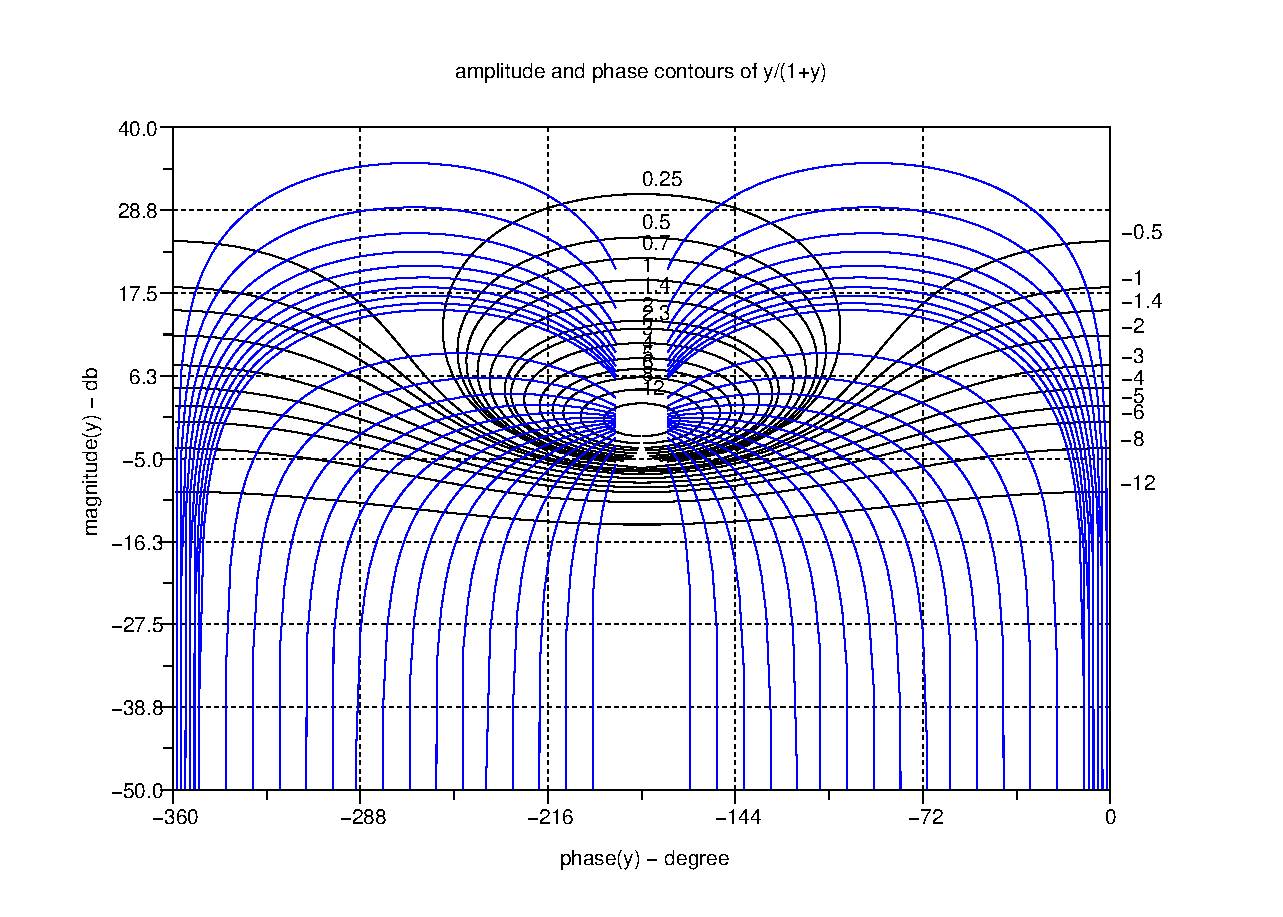
\includegraphics[width=.9\linewidth]{image/nichols_chart.eps}
\end{frame}
\subsection{指标转换}
\label{sec-5-3}
\begin{frame}
\frametitle{系统闭环和开环和频域指标的关系}
\label{sec-5-3-1}

\begin{align*}
G(j\omega) &= Ae^{-j(180^{\circ}-\gamma(\omega))}\\
&=A\left( -\cos\gamma(\omega)-j\sin\gamma(\omega)\right)\\
M&=\left|\frac{G(j\omega)}{1+G(j\omega)}\right| \\
 &=\frac{A}{\sqrt{1+A^2-2A\cos\gamma(\omega)}}\\
 &=\frac{1}{\sqrt{\left[\frac{1}{A}-\cos\gamma(\omega)\right]^2+\sin^2\gamma(\omega)}}\\
M_r &= \frac{1}{\sin\gamma(\omega_r)} \approx \frac{1}{sin\gamma}\qquad (\omega_r \approx \omega_c)
\end{align*}
\end{frame}
\begin{frame}
\frametitle{2阶系统频域指标}
\label{sec-5-3-2}

\begin{align*}
G(j\omega) &= \frac{\omega_n^2}{j\omega(j\omega+2\xi\omega_n)}\\
&=\frac{\omega_n^2}{\omega\sqrt{\omega^2+4\xi^2\omega_n^2}}\angle(-\arctan \frac{\omega}{2\xi\omega_n}-90^{\circ})\\
\omega_c &=\omega_n(\sqrt{4\xi^4+1}-2\xi^2)^{\frac{1}{2}}\\
\gamma &= 180^{\circ}+\angle G(j\omega_c) \\
 &=\arctan \frac{2\xi\omega_n}{\omega_c}
\end{align*}
\end{frame}
\begin{frame}
\frametitle{2阶系统频域指标( $M_r,\omega_r$ )}
\label{sec-5-3-3}

\begin{eqnarray*}
M_r & = &\frac{1}{2\xi\sqrt{1-\xi^2}} \\
\omega_r &=& \omega_n\sqrt{1-2\xi^2}
\end{eqnarray*}
\begin{itemize}
\item <2->$M_r$ 与 $\sigma\%$ 一一对应,且成正比
\end{itemize}
\end{frame}
\begin{frame}
\frametitle{高阶系统频域指标}
\label{sec-5-3-4}
\begin{itemize}

\item 经验公式
\label{sec-5-3-4-1}%
\begin{eqnarray*}
M_r & = & \frac{1}{\sin\gamma}\\
\sigma\% &=& 16\%+0.4(M_r-1), (1\leq M_r\leq 1.8) \\
t_s &=& \frac{K\pi}{\omega_c}\\
K&=& 2+1.5(M_r-1)+2.5(M_r-1)^2 
\end{eqnarray*}

\begin{itemize}
\item <2->$\gamma\uparrow \rightarrow \sigma\%\downarrow \rightarrow \xi\uparrow$
\item <3->$\omega_c\uparrow \rightarrow t_s\downarrow$
\end{itemize}


\item 频域要求:
\label{sec-5-3-4-2}%
\begin{itemize}
\item 低频段:稳态性能
\item 中频段:瞬态性能
\item 高频段:抗干扰能力
\end{itemize}

\end{itemize} % ends low level
\end{frame}

\end{document}
